\subsection{Behavioral effects of dorsomedial striatum pathway inhibition depend on task demand}
\label{sec:glmhmm:2.2.4}
We performed unilateral inhibition of DMS indirect and direct pathways restricted to the cue region (0–200cm) of each task (Fig. 3a,b; laser on 10–20\% of trials; hemisphere of illumination alternated across days). We found that inhibition of the indirect pathway produced a large bias toward contralateral choices during the accumulation of evidence task (Fig. 3c,d), which was significantly greater than that observed in control animals that did not express opsin (Fig. 3e, average contralateral bias: DMS indirect, 42.3\%$\pm$4.4\%, versus no opsin, 5.9\%$\pm$.6\%). Similarly, inhibition of the direct pathway also produced a large choice bias during the accumulation of evidence task (Fig. 3d; average contralateral bias: DMS direct, -36.8\%$\pm$8.6\%), which was also significantly greater than that observed in control animals (Fig. 3e). However, in this case, the direction of the choice bias was in the opposite (ipsilateral) direction to that observed with indirect pathway inhibition (also see Extended Data Fig. \ref{fig:ap1:ext4}a–i for psychometric curves).

Providing a stark contrast to the large effects of pathway-specific DMS inhibition on choice during the evidence accumulation task, inhibition of either pathway had significantly less impact on choice during the ‘no distractors’ and ‘permanent cues’ control tasks (Fig. \ref{fig:glmhmm:3}f–k and Extended Data Fig. \ref{fig:ap1:ext5}a–c; unpaired, two-tailed Wilcoxon rank-sum test of indirect pathway inhibition evidence accumulation versus no distractors, $P=8.0 \times 10^{-4}$, z=3.4, or evidence accumulation versus permanent cues, $P=0.001$, $z=3.3$; and direct pathway inhibition evidence accumulation versus no distractors, $P=0.002$, $z=-3.1$, or evidence accumulation versus permanent cues, $P=0.005$, $z=-2.8$). In fact, the effects of pathway-specific DMS inhibition on choice bias in either control task did not significantly differ from those observed in control animals (Fig. 3h, for ‘no distractors’; Fig. \ref{fig:glmhmm:3}k, for ‘permanent cues’; see also Extended Data Fig. \ref{fig:ap1:ext4}a–i for psychometric curves).

Thus, inhibition of DMS pathways elicited strong and opposing effects on choice in the task with the greatest cognitive demand, which required the accumulation of sensory evidence across multiple seconds to arrive at a decision and had a far limited impact on choice in task variants with reduced cognitive demand.

\begin{figure}[t!]
  \begin{center}
    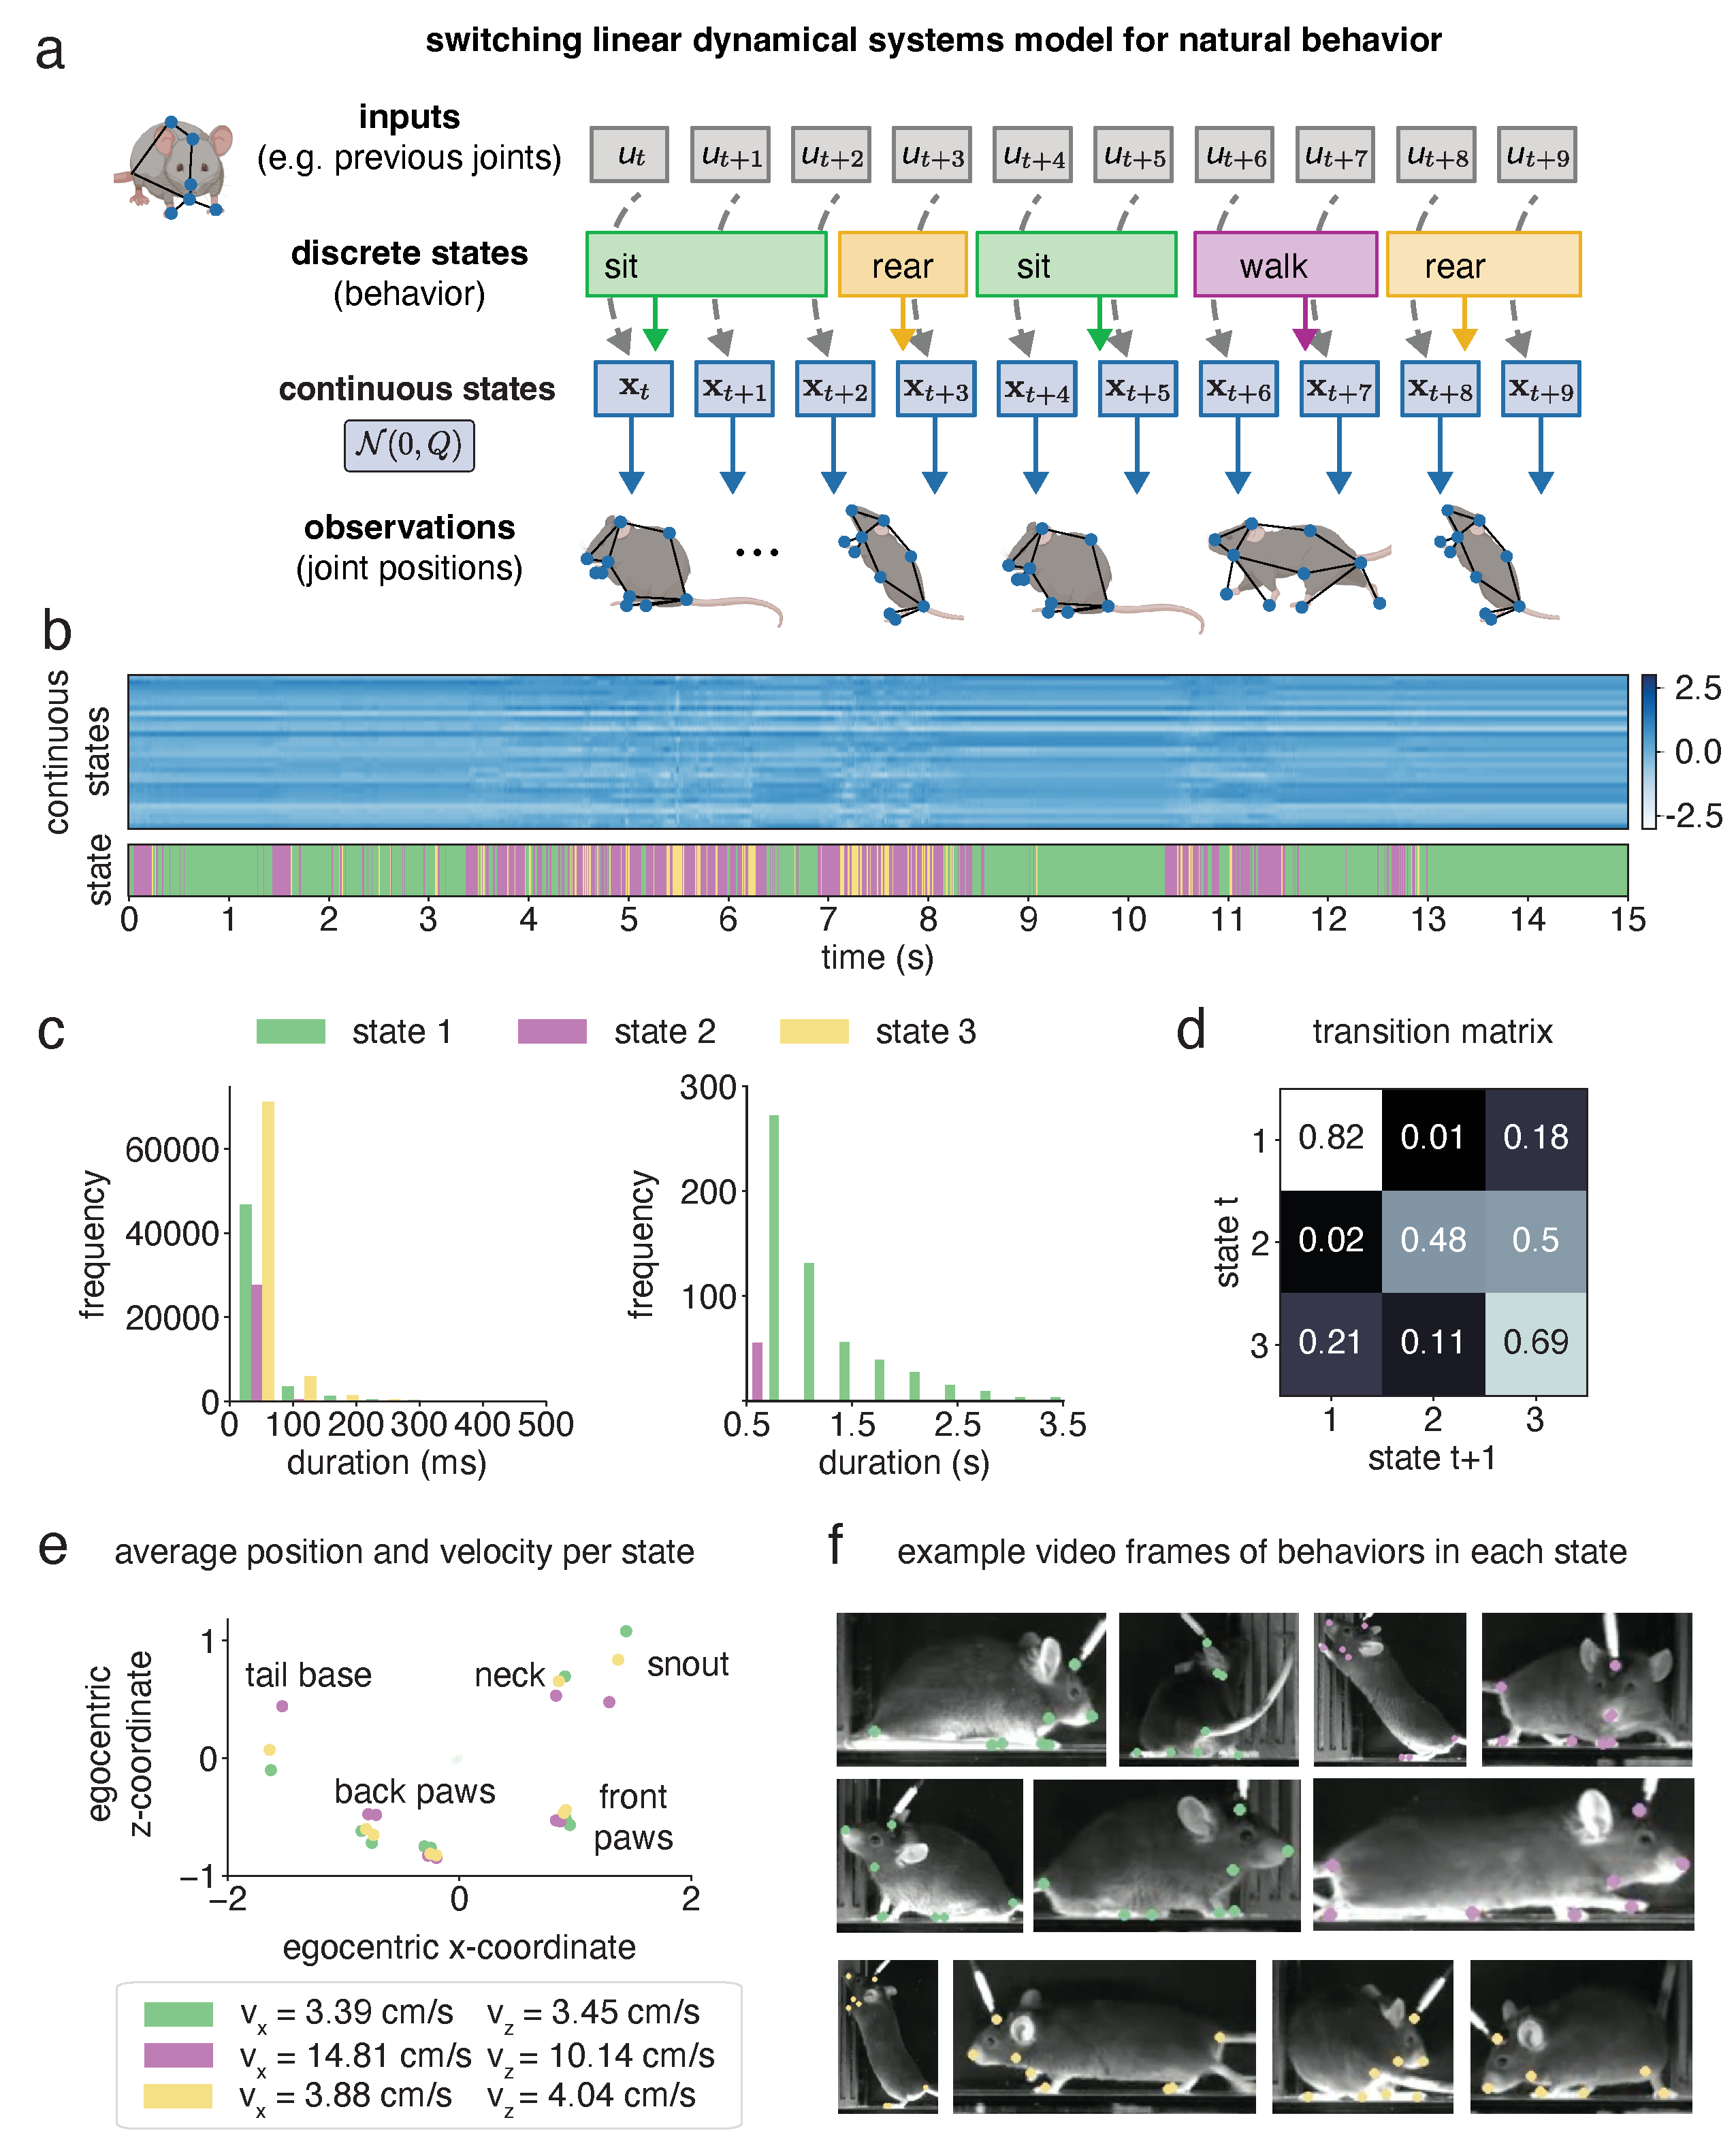
\includegraphics[width=0.90\linewidth]{ch2-glmhmm/glmhmm-figures/Fig3.pdf}
    \caption[Inhibition of DMS but not NAc pathways has strong and opposing influence on choice during an evidence accumulation task, while having weaker effects during task variants with diminished cognitive demands]{\textbf{Inhibition of DMS but not NAc pathways has strong and opposing influence on choice during an evidence accumulation task, while having weaker effects during task variants with diminished cognitive demands.} }
    \label{fig:glmhmm:3}
  \end{center}
  \vspace{-1.5cm}
\end{figure}
\begin{figure}[t!]
  \contcaption{(a) Schematic of bilateral viral delivery of Cre-dependent NpHR to the dorsomedial striatum (DMS). (b) Schematic of bilateral fiberoptic implantation of the DMS and unilateral inhibition in behaving mice, with example histology from a mouse expressing NpHR in the indirect (left, D2R-/A2a-Cre) or direct (middle, D1R-Cre) pathways, or DMS illumination in the absence of NpHR (right, no opsin, A2a-/D2R- or D1R-Cre). 532-nm light (5-mW) was delivered unilaterally to the left or right hemisphere on alternate testing sessions and choice bias contralateral or ipsilateral to the hemisphere of inhibition was quantified. (c) Schematic of the evidence accumulation task with delivery of 532-nm light restricted to the cue region (0-200cm) on a random subset of trials (10-20\%). (d) Average across mouse choice bias during the evidence accumulation task. Choice bias was defined as the difference between percent correct performance on trials when the correct choice was contralateral or ipsilateral to the inhibited hemisphere (\% correct, contralateral-ipsilateral, positive values indicate a contralateral bias). Bias was calculated separately on laser off (black) and laser on (green) trials for mice receiving unilateral indirect pathway inhibition (left, n = 11 mice, n = 16,935 laser off and n = 3,390 laser on trials), unilateral direct pathway inhibition  (middle: n = 10 mice; n = 14,030 laser off and n = 3,103 laser on trials), or unilateral illumination of the DMS in the absence of NpHR (right, n = 11 mice, n = 21,422 laser off and n = 5,113 laser on trials). (e) Difference in contralateral choice bias (\% correct, contralateral-ipsilateral) between laser off and on trials (\% bias, on-off) in mice performing the evidence accumulation task and receiving indirect pathway inhibition, direct pathway inhibition, or DMS illumination in the absence of NpHR. Asterisks indicate significance of unpaired, two-tailed Wilcoxon ranksum comparison of indirect to no opsin: ***p = 1.1x10-4, z = 3.9; direct to no opsin: ***p = 2.2x10-4, z = -3.7). (f-h) Same as c-e but for the no distractors (control 1) task. Indirect: n = 7 mice, n = 13,706 laser off and n = 3,288 laser on trials; direct: n = 9 mice, n = 14,647 laser off and n = 3,682 laser on trials; no opsin: n = 4 mice, n = 3,654 laser off and n = 901 laser on trials. Asterisks indicate significance of unpaired, two-tailed Wilcoxon ranksum comparison of indirect to no opsin: not significant (n.s.), p = 0.22, z = 1.2. Direct to no opsin: not significant (n.s.), p = 0.08, z = -1.8. (i-k) As in c-e but for the permanent cues (control 2) task. Indirect: n = 7 mice, n = 4,033 laser off and n = 929 laser on trials; direct: n = 7 mice, n = 6,061 laser off and n = 1,494 laser on trials; no opsin: n = 6 mice, n = 3,975 laser off and n = 923 laser on trials. Asterisks indicate significance of unpaired, two-tailed Wilcoxon ranksum comparison of indirect to no opsin: not significant (n.s.), p = 0.13, z = 1.5. Direct to no opsin: not significant (n.s.), p = 0.62, z = 0.5. (l) As in a but for bilateral viral delivery of Cre-dependent NpHR to the nucleus accumbens (NAc). (m) Same as b but for bilateral fiberoptic implantation of the NAc and unilateral inhibition in behaving mice, with example histology from a mouse expressing NpHR in the indirect (left, D2R-/A2a-Cre) or direct (middle, D1R-Cre) pathways, or NAc illumination in the absence of NpHR (right, no opsin, A2a-/D2R- or D1R-Cre). (n-p) As in c but for pathway-specific NAc inhibition during the accumulation of evidence task. Indirect: n = 9 mice, n = 11,978 laser off and n = 2,604 laser on trials; direct: n = 10 mice, n = 15,430 laser off and n = 3,348 laser on trials; no opsin: n = 7 mice, n = 9,819 laser off and n = 1,488 laser on trials. Asterisks indicate significance of unpaired, two-tailed Wilcoxon ranksum comparison of indirect to no opsin: not significant (n.s.), p = 0.86, z = 0.18; direct to no opsin: not significant (n.s.), p = 0.04, z = 2.0. Throughout solid bars denote across mouse mean values $\pm$S.E.M. and transparent ‘x’ indicate individual mouse mean. To account for multiple group comparisons we considered p-values significant after Bonferroni correction (2 comparisons).}% Continued caption
\end{figure}

While DMS pathway inhibition had minimal impact on movement in a virtual corridor (Fig. \ref{fig:glmhmm:1} and Extended Data Fig. \ref{fig:ap1:ext2}), we considered the possibility that pathway-specific DMS inhibition altered motor performance in the T-mazes. We found no cross-task differences in the effects of pathway-specific inhibition on measures of velocity, distance traveled or per-trial standard deviation in view angle (Extended Data Fig. \ref{fig:ap1:ext6}a–i). However, we found subtle but opposing effects of pathway-specific inhibition on average x-position and view angle (Extended Data Fig. \ref{fig:ap1:ext6}j–k) in the evidence accumulation task. The direction of these biases was similar in the control tasks, but consistently smaller than in the evidence accumulation task. Thus, in line with the close relationship between x-position/view angle and choice in the absence of inhibition in each task (Extended Data Fig. \ref{fig:ap1:ext3}g–j), pathway-specific DMS inhibition produced the same general pattern of cross-task effects on choice bias (Extended Data Fig. \ref{fig:ap1:ext5}b–d) and x-position/view angle (Extended Data Fig. \ref{fig:ap1:ext6}j,k). As the quantitative relationship between x-position or view angle and choice is indistinguishable across tasks in the absence of neural inhibition (Extended Data Fig. \ref{fig:ap1:ext3}g–j), cross-task differences in motor strategy do not provide a trivial explanation for these effects. Rather, taken together with the absence of an effect of pathway-specific DMS inhibition on motor output in the virtual corridor (Fig. \ref{fig:glmhmm:1}h,i), these data imply that the effects of inhibition on behavior depend on cognitive demands.